\begin{figure}[H]
\centering
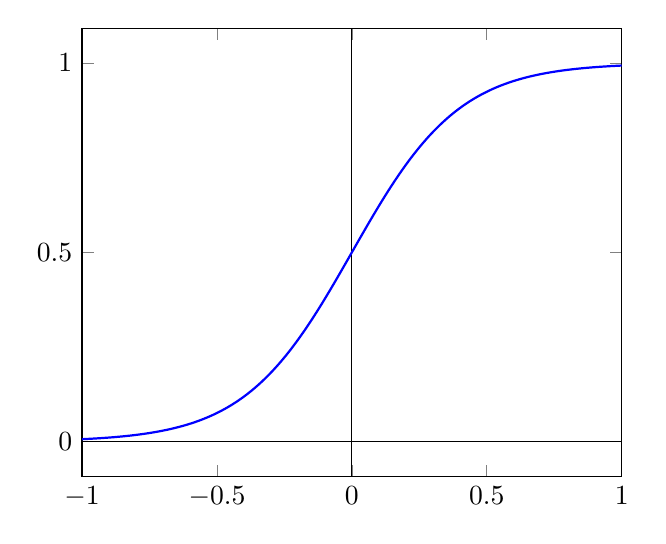
\begin{tikzpicture}
    \begin{axis}[
    	xmin=-1,
        xmax=1,
        ytick distance=0.5
        ]
		\draw[line width=0mm,] 
        (axis cs:\pgfkeysvalueof{/pgfplots/xmin},0) -- 
        (axis cs:\pgfkeysvalueof{/pgfplots/xmax},0);
        
		\draw[line width=0mm] 
        (axis cs:0,\pgfkeysvalueof{/pgfplots/ymin}) -- 
        (axis cs:0,\pgfkeysvalueof{/pgfplots/ymax});

      % plot the stirling-formulae
      \addplot[mark=none, thick, domain=-2:2, blue,samples=500]
      	{1/(1+exp(-5*x))};
    \end{axis}
\end{tikzpicture}

\caption{Sigmoid activation function.}
\label{fig:sigmoid}
\end{figure}